%!TEX root = labo.tex
\setcounter{chapter}{0}
\chapter{Basic Configurations}

The goal of the first lab is to make you acquainted with the hardware and software needed to perform the tasks in other modules. Furthermore we will have a look at the various sniffing possibilities in wireless networks.

\section{Device Exploration}

Have a closer look a the devices used for this course. 

\begin{exercise}{Getting to know the interfaces}
	\begin{enumerate}
		\item Log in on \ac{wmn}1. \newline
		\command{ssh root@wmn1}
		\item When asked to give a name, enter
		\command{AP}
		\item Get a list of all available interfaces. \newline
		\command{\prompt{\acs{ap}} ifconfig -a}
		\item List the interfaces and their \ac{mac} addresses.\newline		\begin{esolution}
		\end{esolution}
		\item A \ac{mac} address is unique per card, but also carries a generic part, identifying the vendor of a card. List the prefixes and find out the vendors (name) of all different interfaces found in the node.\\
		\remark Google is your friend!\newline		
		\begin{esolution}
		\end{esolution}
	\end{enumerate}
	
\end{exercise}

\section{Access Point Setup}

\begin{figure}[h]
	\begin{center}
		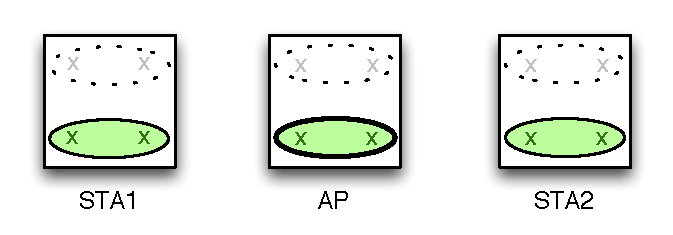
\includegraphics[width=0.8\textwidth]{images/snif1.pdf} 
		\caption{The basic infrastructure setup}
		\label{fig:basic-infra}  
	\end{center}
\end{figure}

The goal is to create a basic infrastructure setup as can be found at home. The setup consists of one \ac{ap} and two connected stations as shown in figure \ref{fig:basic-infra}. In this case, two laptops are connected to the same \ac{ap} and can communicate to each other. We will not consider any communication to the outside world.

\subsection{\ac{ap} Configuration}
To set up this basic infrastructure network, start by configuring the \ac{ap}.

\begin{exercise}{Set up an \ac{ap}}
\begin{enumerate}
	\item Check the wireless parameters of wlan1:\newline
	\command{\prompt{\acs{ap}} iwconfig wlan1}\newline
	This should give you some output like
\begin{verbatim}
wlan1     IEEE 802.11abgn  ESSID:off/any  
          Mode:Managed  Access Point: Not-Associated   Tx-Power=0 dBm   
          RTS thr:off   Fragment thr:off
          Encryption key:off
          Power Management:off
\end{verbatim}

\remark Remark that we did not configure the interface yet!

Give an explanation for all available parameters which are displayed using \incommand{iwconfig} (hint: man pages).\newline
\begin{esolution}
\end{esolution}


\item Configure the wlan1 interface using your assigned channel and the \ac{essid}:\newline
\begin{lstlisting}
interface=wlan
driver=nl80211
logger_syslog=-1
logger_syslog_level=2
logger_stdout=-1
logger_stdout_level=2
debug=4
hw_mode=a
channel=x
macaddr_acl=0
auth_algs=3
eapol_key_index_workaround=0
eap_server=0
wpa=0
ssid=wmn-gid-A
\end{lstlisting}

This file can be found on the devices as \texttt{hostapd.conf}. Edit it to change the channel number, interface name and \ac{essid}, and then perform the following:\newline
\command{\prompt{\acs{ap}} hostapd -B hostapd.conf}

\incommand{\prompt{\acs{ap}} iwconfig} should now return something like: 
\begin{verbatim}
wlan1     IEEE 802.11abgn  Mode:Master  Tx-Power=20 dBm   
          RTS thr:off   Fragment thr:off
          Power Management:off
\end{verbatim}

\end{enumerate}
\end{exercise}

\subsection{Station Configuration}

\begin{exercise}{Configuring the wireless stations}
	
We will now configure \emph{both} stations  and verify they get associated with the \ac{ap} you just created. Make sure to repeat the commands to configure the second station.

\begin{enumerate}
	\item Bring up the interface: \newline
	\command{\prompt{\acs{sta}1} ifconfig wlan1 up}
	\item Configure the interface to connect to our \ac{ap}: \newline
	\command{\prompt{\acs{sta}1} iw dev wlan1 connect \ac{wmn}-\acs{gid}-A}
	\item Do the same on \ac{sta}2.



\remark When you run \incommand{iwconfig}, the \incommand{Access Point} parameter should show the \ac{mac} address of the \ac{ap} and show identical frequencies and \acp{essid} on both stations. 
\begin{verbatim}
wlan1     IEEE 802.11abgn  ESSID:"wmn-0-A"  
          Mode:Managed  Frequency:5.24 GHz  Access Point: 00:00:11:22:33:44   
          Bit Rate=1 Mb/s   Tx-Power=5 dBm   
          RTS thr:off   Fragment thr:off
          Encryption key:off
          Power Management:off
          Link Quality=12/70  Signal level=-164 dBm  
          Rx invalid nwid:0  Rx invalid crypt:0  Rx invalid frag:0
          Tx excessive retries:0  Invalid misc:4   Missed beacon:0
\end{verbatim}
	\item What parameters are different in your output compared to the output above?\newline
	\begin{esolution}
	\end{esolution}
\end{enumerate}
\end{exercise}

If the output for both stations confirms the association between the two wireless stations and the \ac{ap}, the actual L2 connection between these three devices is up and running. To verify the connection, we will configure IP addresses on the stations and have them communicate.

\begin{exercise}{Verifying the basic setup}\label{ex:pingtest}
	
	\begin{enumerate}
		\item Configure the IP address of \ac{sta}1 and \ac{sta}2:\newline
		\command{\prompt{\ac{sta}1} ip addr add fc00::\acs{gid}::1/64 dev wlan1}
		\command{\prompt{\ac{sta}2} ip addr add fc00:\acs{gid}::2/64 dev wlan1}
		\item Start a ping session from \ac{sta}1 to \ac{sta}2. Give the minimum, maximum and average \ac{rtt}:\newline
		\command{\prompt{\ac{sta}1} ping6 -c 30 fc00:\acs{gid}::2}
		\begin{esolution}
		\end{esolution}
		\item Perform a ping between the same devices as before, but this time, use the wired IP addresses. Again write down the same values.\newline
		\begin{esolution}
		\end{esolution}
	\end{enumerate}
\end{exercise}

\remark Remark that we did not (yet) enable L3 capabilities at the \ac{ap}.


\section{Wireless Sniffing}

Using the basic network we constructed in the previous section, we will go through the various sniffing modes available in wireless networks. The main difference between wired and wireless networks is obviously the fact that the transmission medium (radio waves vs. cable) is shared amongst all wireless users. Therefore, sniffing the network offers a lot more opportunities in wireless systems.
\begin{figure}
	\begin{center}
		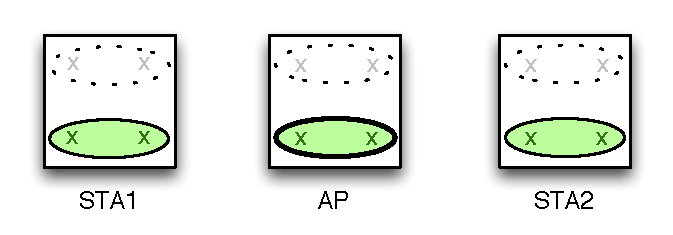
\includegraphics[width=0.5\textwidth]{images/snif1.pdf} 
		\caption{Wireless packet capture setup} 
		\label{fig:snif1} 
	\end{center}
\end{figure}


The first setup is shown in figure \ref{fig:snif1} and corresponds to the basic setup we created in the previous section. 



\begin{exercise}{First scan}\label{ex:firstScan}
\begin{enumerate}
	\item Make sure the \ac{nd} cache of both \acp{sta} is cleared.\label{ex:1-1}\newline
	\command{\prompt{\ac{sta}2} ip neigh flush dev wlan1}
	\command{\prompt{\ac{sta}1} ip neigh flush dev wlan1}
	\remark You can always check the state of the cache using \command{ip neigh show}
	\item On the \ac{ap} and on both \acp{sta}, start a packet capture using \incommand{tcpdump} and save it to \file{snif-location.pcap}. \newline
	\remark This is the time to make sure that you have a remote location mounted with \verb!sshfs! in /mnt!\newline\newline
	\command{\prompt{\acs{ap}} tcpdump -i wlan1 -w \file{\acs{ap}.pcap}}
	\command{\prompt{\acs{sta}1} tcpdump -i wlan1 -w \file{\acs{sta}1.pcap}}
	\command{\prompt{\acs{sta}2} tcpdump -i wlan1 -w \file{\acs{sta}2.pcap}}
	\item Start a ping session from \ac{sta}1 to \ac{sta}2. Limit the ping to only two requests. \label{ex:1-3}\newline
	\command{\prompt{\ac{sta}1} ping6 -c 2 fc00:\acs{gid}::2} 
	\item Which type of packets can be seen in the \acs{ap} trace file? You can open the trace file with wireshark on the remote computer.\newline
	\begin{esolution}
	\end{esolution}
	\item Now, take a closer look at the \ac{mac} headers. Which type of link layer headers show up on the packets?\newline
	\begin{esolution}
	\end{esolution}
\end{enumerate}
\end{exercise}


From the tracefile made on the AP, it is impossible to see if we made a wired or wireless trace. Let's more closely examine the tracefiles made on the stations, where a difference will become apparent.

\begin{exercise}{Scanning other interfaces}\label{ex:scan}

Open the trace files made on both the sending and receiving station.
	
	\begin{enumerate}
		\item You should observe duplicate entries. Describe which duplicates are observed in each file (use packet numbers!):\newline
		\begin{esolution}
		\end{esolution}
		\item Take a closer look at the \ac{mac} addresses of the duplicate packets using Wireshark. What addresses are used on the frames? Are they identical?\newline
		\begin{esolution}
		\end{esolution}
	\end{enumerate}
\end{exercise}

\incommand{tcpdump} will automatically put the interface in \emph{promiscuous mode}. This means all packets which can be read by the wireless interface will be delivered up the networking stack even though the destination \ac{mac} address does not correspond to the address of the specific card. Each interface receives all packets sent by the \ac{ap}. If the destination \ac{mac} address is not that of the receiving interface, the packet is normally dropped. In promiscuous mode, however, these packets are nevertheless stored in the trace file. Now repeat the previous exercise but disable the promiscuous mode.

\begin{exercise}{Disabling promiscuous mode}


\begin{enumerate}
	\item Make sure the \ac{nd} cache is cleared on \ac{sta}1 and \ac{sta}2. \newline 
	\command{\prompt{\acs{sta}1} ip neigh flush dev wlan1}
	\command{\prompt{\acs{sta}2} ip neigh flush dev wlan1} 
	\item On \ac{sta}1, start a packet capture not using promiscuous mode using \incommand{tcpdump} and save it to \file{\acs{sta}1.pcap}.\newline
	\command{\prompt{\acs{sta}1} tcpdump -i wlan1 -p -w \file{\acs{sta}1.pcap}} 
	\item Start a ping session from  \ac{sta}2 to \ac{sta}1. \newline
	\command{\prompt{\acs{sta}2} ping6 -c 2 fc00:\acs{gid}::1} 
	\item Do you still observe the duplicate entries?\newline
	\begin{esolution}
	\end{esolution} 
\end{enumerate}
\end{exercise}

\begin{figure}[h]
	\begin{center}
		\subfloat[]{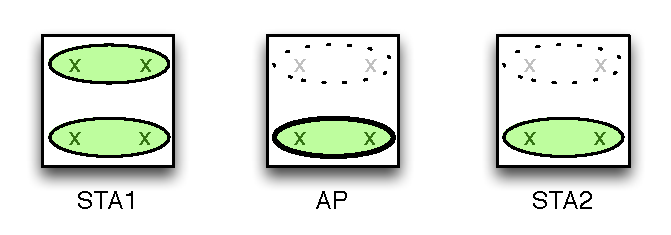
\includegraphics[width=0.5\textwidth]{images/snif2b.pdf} 	\label{fig:snif2b} }
		\subfloat[]{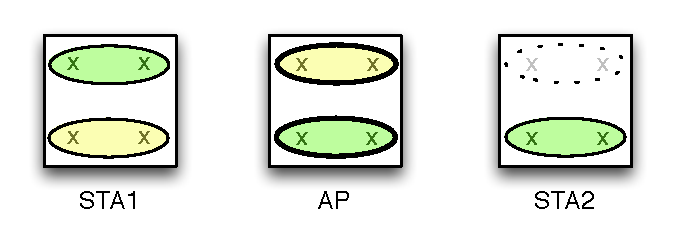
\includegraphics[width=0.5\textwidth]{images/snif2c.pdf} 	\label{fig:snif2c} }
		\caption{Third party scanning} 
	
	\end{center}
\end{figure}

\begin{exercise}{Third party scanning}
	\label{ex:secondAP}
	
So far, we only sniffed the network on nodes which took part of the network activity. Let's introduce another party, which just wants to listen to what is happening on the channel. Imagine a notebook eavesdropping on the traffic of a wireless cell. First we will add it to the same \ac{essid} and later on change it to a different \ac{essid}.  The intended setups are shown in figure \ref{fig:snif2b} and \ref{fig:snif2c}. The first situation then compares to a situation where a laptop is connected to your home network and is sniffing the traffic of other active stations in this network, while the latter situation can be seen as you being connected to your network, trying to sniff the network of a neighbour on the same channel, but using a different network name.
	
	We'll start from the previous setup.\newline
	\remark It is essential that you bring \incommand{wlan1} down on \ac{sta}1 first. 

	\begin{enumerate}
		\item Bring \incommand{wlan1} down on \ac{sta}1.\newline
		\command{\prompt{\ac{sta}1} ifconfig wlan1 down}
		\item Add \incommand{wlan0} of \ac{sta}1 to get the setup of \ref{fig:snif2b}: \newline
		\command{\prompt{\ac{sta}1} ifconfig wlan0 up}
		\command{\prompt{\ac{sta}1} iw dev wlan0 connect essid wmn-\acs{gid}-A}
		\command{\prompt{\ac{sta}1} ip addr add fc00:grID::1/64 dev wlan0}
		\item Now, reintroduce \incommand{wlan1} of \ac{sta}1 to the network.\newline
		\command{\prompt{\ac{sta}1} ifconfig wlan1 up}
		\command{\prompt{\ac{sta}1} iw dev wlan1 connect wmn-\acs{gid}-A}
		\item Configure \incommand{wlan1} with the following IP address:\newline
		\command{\prompt{\ac{sta}1} ip addr add fc00:grID:1::1/64 dev wlan1}
		\remark Remark that this IP address belongs to a different subnet! This is in preparation of the next part of the exercise.
		\item Repeat steps \ref{ex:1-1} to \ref{ex:1-3} from exercise \ref{ex:firstScan} , but in step 2, start the capture only on \incommand{wlan1} of \ac{sta}1 and save it to \file{\acs{sta}1.A.pcap}.
		\item To change the \verb!wlan1! interface to another \ac{essid}, we first need another \ac{ap} managing this \ac{essid} (figure \ref{fig:snif2c}). Configure a second \ac{ap} interface on the \ac{ap} node, this time using ``\ac{wmn}-\ac{gid}-B'' as essid\\
		\remark Copy the previous hostapd.conf file and change the ssid and interface.
		\item Make sure \verb!wlan1! of \ac{sta}1 is connected to the \ac{wmn}-\ac{gid}-B network.
		\item Repeat the same exercise again, saving the trace to \file{\acs{sta}1.B.pcap}. \newline
		\item Compare the results from both tests. How do these two setups compare to a wired setup?\newline
		\begin{esolution}
		\end{esolution}
	\end{enumerate}
	
\end{exercise}


\begin{exercise}{Pinging the \ac{ap}}

In the previous exercises, we have used the \ac{ap} only as a L2 device. The \ac{ap} can of course also be configured as a L3 device. We will now configure the \ac{ap} as a L3 device and perform the same ping test again, but this time from \ac{sta}1 to \ac{ap}.
	\begin{enumerate}
		\item Add an IP address on \incommand{wlan0} of the \ac{ap}: \newline
		\command{\prompt{\ac{ap}} ip addr add fc00:grID:1::3/64 dev wlan0}
		\item On \ac{sta}1, start a packet capture on \incommand{wlan1} and save it to \file{\acs{sta}1.pcap}. \newline
		\command{\prompt{\ac{sta}1} tcpdump -i wlan1 -w \file{\acs{sta}1.pcap}} 
		\item Start a ping session from \ac{sta}1 to \ac{ap}. Limit the ping to only two requests. \label{ex:1-3}\newline
		\command{\prompt{\ac{sta}1} ping6 -c 2 fc00:grID:1::3} 
		\item In the trace files, do you observe duplicate entries? Why or why not?\newline
		\begin{esolution}
		\end{esolution}
	\end{enumerate}

\end{exercise}


\begin{exercise}{Sniffing in monitor mode}

\begin{figure}[h]
	\begin{center}
		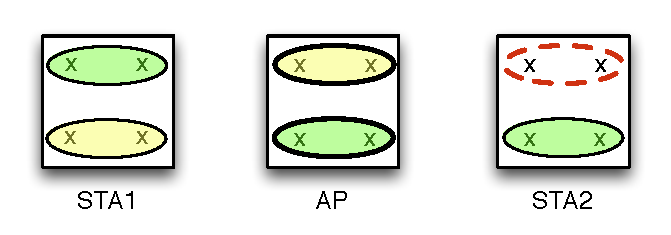
\includegraphics[width=0.5\textwidth]{images/snif4.pdf} 
		\caption{Introducing a monitoring interface.}
		\label{fig:snif4} 
	\end{center}
\end{figure}

Until now, not much difference has been observed compared to network sniffing on a wired network - apart from observing duplicate packets. In the next exercises we will broaden the setups to show the actual differences. Firstly, the monitor interface will be introduced. Configuring a \acl{wnic} in monitor mode will enable you to see all traffic that is present in a certain channel. In figure \ref{fig:snif4} the next setup is shown. We continue from the previous setup and add an extra interface.
\begin{enumerate}
	\item Configure the monitoring device:\newline
	\command{\prompt{\ac{sta}2} iw dev wlan0 set type monitor}
	\item Bring the monitor interface up: \newline
	\command{\prompt{\ac{sta}2} ifconfig wlan0 up} 
	\item Configure the channel: \newline
	\command{\prompt{\ac{sta}2} iw dev wlan0 set channel x} 
	\remark Remark that it is not necessary to configure an \ac{essid}. Why?\newline
	\begin{esolution}
	\end{esolution}
	\item Clear the \ac{nd} caches:\newline
	\command{\prompt{\ac{sta}2} ip neigh flush dev wlan1}
	\command{\prompt{\ac{sta}1} ip neigh flush dev wlan0} 
	\item Start a capture session on the monitor interface and save it to \file{\acs{sta}2.pcap}:\newline
	\command{\prompt{\ac{sta}2} tcpdump -i wlan0 -w \file{\acs{sta}2.pcap}} 
	\item Start a ping session from \ac{sta}1 to \ac{sta}2. \label{ex:3-4}\newline
	\command{\prompt{\ac{sta}1} ping6 -c 2 fc00:\acs{gid}::2} 
	\item Open the capture file in Wireshark. 
	\begin{itemize}
		\item What type of frames are visible within the trace? Give an example (packet number) of each. \newline
		\begin{esolution}
		\end{esolution}
		\item What type of link layer headers  are visible now?\newline
		\begin{esolution}
		\end{esolution}
		\item A radiotap header should also be visible before the link layer header. This header is not actually transmitted, but is used to communicate transmission statistics between the driver and kernel. As such, it reports on various transmission statistics as the signal strength and the used antenna. Select a packet (give the packetID within the trace), and list which items are present. Although the format is standardized, the actual content depends on the driver and hardware used.\newline
		\begin{esolution}
		\end{esolution}
		\item Describe the path a packet takes to be delivered from one \acl{sta} to another. Give a detailed overview of the various addresses in the headers. Identify the frames (packet ID) from the trace you use to illustrate this.\newline
		\begin{esolution}
		\end{esolution}
	\end{itemize}
\end{enumerate}
\end{exercise}


Remember the traces you made containing duplicate packets? The duplicates can now be clearly observed in the traces from a monitor interface. Each transmission from one \acl{sta} to another, both connected to the same \ac{ap} is always relayed over the \ac{ap}. The sender thus first recorded its transmission and then detected the relayed frame on the air. Frames which are sent to an \ac{ap}, are discarded by other stations. This explains why a third station did not show duplicate packets. Finally, an \acl{ap} will only report one occurrence in \incommand{tcpdump} traces, as the relaying of a frame is done transparently to the kernel in the hardware/driver.


\begin{exercise}

Finally, we will repeat exercise \ref{ex:secondAP}. We will be sending traffic on both wireless networks and monitor the channel. The setup remains unchanged (see figure \ref{fig:snif4}).

\begin{enumerate}
	\item Clear the \ac{nd} caches as before. Be sure to delete all \ac{nd} entries on all \acp{wnic}!
	\item Start a scan on the monitor interface of \ac{sta}2 and save it to \file{\acs{sta}2.pcap}: \newline
	\command{\prompt{\ac{sta}2} tcpdump -i wlan0 -w \file{\acs{sta}2.pcap}}
	\item Perform a ping from \ac{sta}1 to \ac{ap} and start a ping from \ac{sta}2 to \ac{sta}1, both on \incommand{wlan1}. This means we will inject traffic on both wireless networks.\newline
	\remark These pings can be performed consecutively. Make sure they are in the same capture session. \newline
	\command{\prompt{\ac{sta}1} ping6 -c 2 fc00:\acs{gid}:1::3}
	\command{\prompt{\ac{sta}2} ping6 -c 2 fc00:\acs{gid}::1}
	\item Which ping session(s) is/are visible in the trace?\newline
	\begin{esolution}
	\end{esolution}
\end{enumerate}




\end{exercise}





\section{Ad-Hoc Networks}

In the next section, we will set up a basic ad-hoc network. Contrary to the infrastructure network we used in the previous section, ad-hoc networks are built from identically configured hosts, without a central entity in charge. Let's start right away to build our first ad-hoc network.

\begin{exercise}{Basic ad-hoc network}

\begin{enumerate}
	\item To ensure all interfaces are in the default state, reboot all devices:\newline
	\command{\prompt{\ac{ap}} reboot}
	\command{\prompt{\ac{sta}1} reboot}
	\command{\prompt{\ac{sta}2} reboot}
	\item  The basic setup is shown in figure \ref{fig:ad-hoc1}. All nodes will have the same configuration: mode, \ac{essid} and channel.\newline
	\command{\prompt{\ac{sta}1} iw dev wlan1 set type ibss}
	\command{\prompt{\ac{sta}2} iw dev wlan1 set type ibss}
	\command{\prompt{\ac{sta}3} iw dev wlan1 set type ibss}
	\begin{figure}
		\begin{center}
			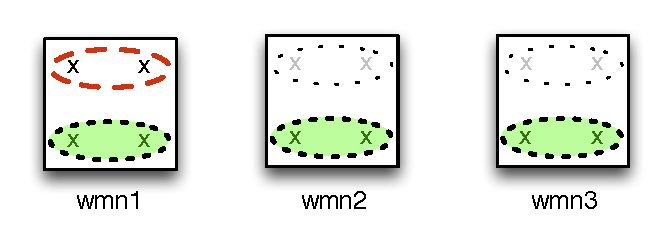
\includegraphics[width=0.5\textwidth]{images/adhoc1.pdf} 
			\caption{Basic ad-hoc network.}
			\label{fig:ad-hoc1} 
		\end{center}
	\end{figure}
	\item Assign IP addresses to all interfaces and activate them:\newline
	\command{\prompt{\ac{sta}1} ip addr add fc00:\acs{gid}::1/64 dev wlan1}
	\command{\prompt{\ac{sta}2} ip addr add fc00:\acs{gid}::2/64 dev wlan1}
	\command{\prompt{\ac{sta}3} ip addr add fc00:\acs{gid}::3/64 dev wlan1}
	\command{\prompt{\ac{sta}1} ifconfig wlan1 up}
	\command{\prompt{\ac{sta}2} ifconfig wlan1 up}
	\command{\prompt{\ac{sta}3} iwconfig wlan1 up}
	\item Configure all interfaces with a \ac{essid} and a channel:\newline
	\command{\prompt{\ac{sta}1} iw dev wlan1 ibss join \ac{wmn}-\acs{gid}-A <frequency>}
	\command{\prompt{\ac{sta}2} iw dev wlan1 ibss join \ac{wmn}-\acs{gid}-A <frequency>}
	\command{\prompt{\ac{sta}3} iw dev wlan1 ibss join \ac{wmn}-\acs{gid}-A <frequency>}
	\remark The frequency you should use here can be found in the introduction section.\newline
	\item To monitor the traffic in the channel, set up a monitor interface on \ac{sta}1:\newline
	\command{\prompt{\ac{sta}1} iw dev wlan0 set type monitor}
	\command{\prompt{\ac{sta}1} ifconfig wlan0 up}
	\command{\prompt{\ac{sta}1} iw dev wlan0 set freq <frequency>}
	\item Scan using the monitor interface and save it to \file{\acs{sta}1.pcap}.\newline
	\command{\prompt{\ac{sta}1} tcpdump -i wlan0 -w \file{\acs{sta}1.pcap}}
	\item Verify that the nodes now all can reach each other:\newline
	\command{\prompt{\ac{sta}1} ping6 -c 2 fc00:\acs{gid}::2}
	\command{\prompt{\ac{sta}2} ping6 -c 2 fc00:\acs{gid}::3}
	\command{\prompt{\ac{sta}3} ping6 -c 2 fc00:\acs{gid}::1}	
	\item Describe how data is exchanged between the various hops. How does this compare to infrastructure mode? Motivate your findings by selecting frames (give the packet ID) from the trace file and describe their \ac{mac} header and addressing scheme.\newline
	\begin{esolution}
	\end{esolution}
	
	\item Repeat the ping tests from exercise \ref{ex:pingtest} (from \ac{sta}1 to \ac{sta}2 and write down the requested values. Do you observe a significant change in timings?\newline
	\begin{esolution}
	\end{esolution}
\end{enumerate}
	
\end{exercise}